\section{Main Algorithm}

\subsection{ChartToExpression}
\subsubsection{表达式转化}
	首先,我们需要将含字母的表达式转换为只含有数字的表达式,以便后续计算。
	
	核心代码如下:
	\lstinputlisting{sources/algo_part0.txt}
	\begin{itemize}
		\item	首先,遍历输入的字符串,对于每一个字母,用$loc[]$数组记下它出现的位置
		\item	然后,我们使用变量$mask$来遍历$2 ^ n$种可能输入。由于输出格式的要求,我们采用倒序遍历,即从$2^n - 1$开始,到$0$结束。当$mask$值一定时,对于每一位$i$,可以用位运算$value = (mask >> i) \& 1$来得到第$i$个变量的值$value$。
		\item	得到第$i$个变量的值$value$之后,通过遍历$loc[i]$数组,就可以得到该变量所有出现的位置,从而进行替换。
		\item	由于变量只有$A - H$,取值也只有$0 - 1$,都只有一位,所以直接赋值即可。于是完成了从含字母表达式到纯数字表达式的转换。
	\end{itemize}
\subsubsection{表达式求值}
\paragraph{中缀转后缀\\}
	\subparagraph{中缀表达式与后缀表达式}
		\begin{itemize}
			\item{中缀表达式\\} 
			中缀表示法是算术表达式的常规表示法。称它为中缀表示法是因为每个操作符都位于其操作数的中间,这种表示法只适用于操作符恰好对应两个操作数的时候(在操作符是二元操作符如加、减、乘、除以及取模的情况下)。

			Syntax: operand1 operator operand2
			
			Example: (A+B)*C-D/(E+F)
			
			\item{后缀表达式\\}
			在后缀表示法中,操作符严格位于操作数后面。因其使表达式求值变得轻松,所以被普遍使用。

			Syntax  : operand1 operand2 operator
			
			Example : AB+C*DEF+/-
			\item	由于中缀表示法是书写表达式的常见方式,而后缀表达式更便于计算表达式的值,因此我们常常采用将中缀表达式转化为后缀表达式再求值的方法。
		\end{itemize}
	\subparagraph{具体算法\\}
	中缀转换为后缀的难点在于操作符的优先级处理。由于后缀的操作符紧跟在操作数后,我们可以用一个栈来存储操作符,具体流程如下:
	\begin{itemize}
		\item	初始化一个空堆栈,将结果字符串变量置空。
		\item	从左到右读入中缀表达式,每次一个字符。
		\item	如果字符是操作数,将它添加到结果字符串。
		\item	如果字符是个操作符,弹出操作符,直至遇见左括号、优先级较低的操作符或者同一优先级的右结合符号。把这个操作符压入堆栈。
		\item	如果字符是个左括号,把它压入堆栈。
		\item	如果字符是个右括号,在遇见开括号前,弹出所有操作符,然后把它们添加到结果字符串。
		
		\item	如果到达输入字符串的末尾,弹出所有操作符并添加到结果字符串。
	
	\end{itemize}
	
	Project中,用$InfixToPostfix$函数实现:
	\lstinputlisting{sources/algo_part1.txt}	
\paragraph{后缀表达式求值\\}
	对后缀表达式求值比直接对中缀表达式求值简单。在后缀表达式中,不需要括号,而且操作符的优先级也不再起作用了。
	
	具体算法如下:

	\begin{itemize}
		\item	初始化一个空堆栈
		\item	从左到右读入后缀表达式
		\item	如果字符是一个操作数,把它压入堆栈。
		\item	如果字符是个操作符,弹出两个操作数,执行对应操作,然后把结果压入堆栈。
		
		如果不能够弹出两个操作数,后缀表达式的语法就不正确。
		\item	到后缀表达式末尾,从堆栈中弹出结果。若后缀表达式格式正确,那么堆栈应该为空。
	\end{itemize}

	Project中,用$SolvePostfix$函数实现:
	\lstinputlisting{sources/algo_part2.txt}	

\subsection{ExpressionToChart}
\subsubsection{Quine–McCluskey算法}
	Quine–McCluskey算法是最小化布尔函数的一种方法。它在功能上等同于卡诺图,但是它具有文字表格的形式,因此它更适合用于电子设计自动化算法的实现,并且它还给出了检查布尔函数是否达到了最小化形式的确定性方法。
	
	Quine–McCluskey算法的基本步骤如下:
	\begin{itemize}
		\item{STEP 1\\}	
			将表达式中的最小项用他们的等价二进制数表示
		\item{STEP 2\\}
			将最小项根据它们所含的1的个数进行分组,形成一张最小项表。
			
			如第一组为不含1的,第二组中每个含一个1,以此类推
		\item{STEP 3\\}
			将每个最小项$i$与它下一组的所有最小项$j$进行比较。显然,$j$会比$i$多一个1。
			
			如果$i$与$j$只有一位$b$不同(包括任意项),标记这两个最小项配对成功,将$b$位标记为任意项。
			
			将合并后的新最小项加入新的最小项表中。
			
		\item{STEP 4\\}
			对于每一次形成的新最小项表,重复STEP 3,直到不能产生任何的新配对。
		
		\item{STEP 5\\}
			每一步剩下未配对的即为质蕴涵。(但并不是必要质蕴涵)
	\end{itemize}
	
	\begin{figure}[h]
		\centering
		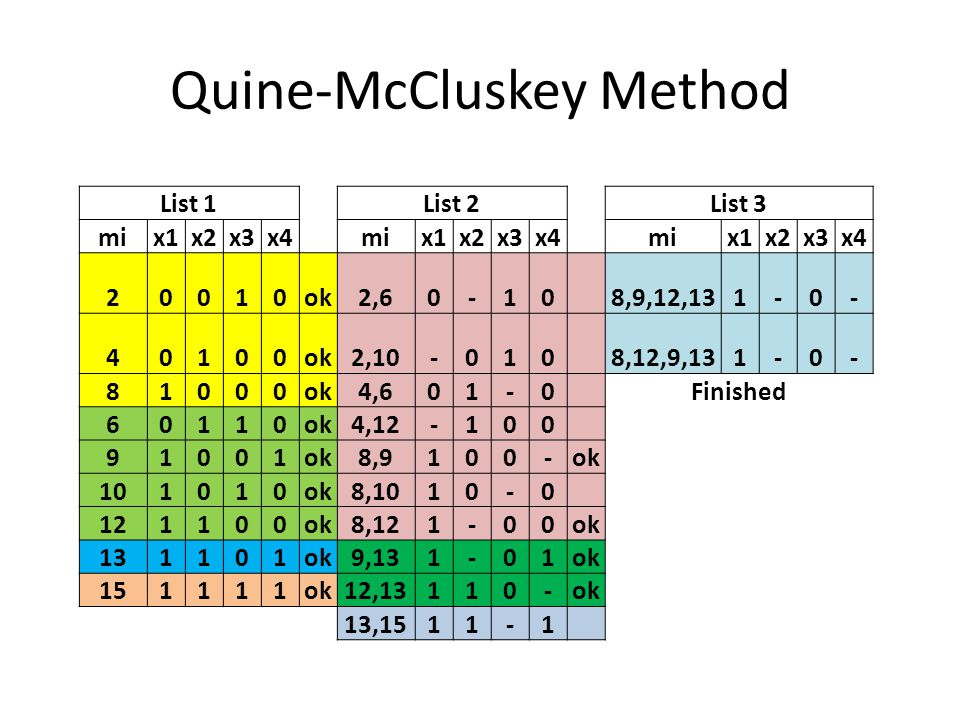
\includegraphics[scale=0.5]{images/QM.jpg}
		\caption{最小项表}
	\end{figure}
	
	由于Quine–McCluskey算法的描述比较清晰,按描述模拟即可。
	
	\lstinputlisting{sources/algo_part3.txt}	

\subsubsection{化简}
	常用方法是petrick化简
	
	这种方法的时间复杂度为$O((2^n)^2)$,由于$n \le 8$,因此时间复杂度不会超过$2 ^ {16} = 65536$,是完全可以接受的
	
	\lstinputlisting{sources/algo_part5.txt}	
